\documentclass[12pt,a4paper]{article}
%\usepackage[utf8]{inputenc}
%\usepackage[portuguese]{babel}
\usepackage{amsmath, amsfonts, amssymb, mathrsfs}
\usepackage{graphicx}
\usepackage{newtxmath}
\usepackage[utf8]{inputenc} % Permite utilizar caracteres especiais: Ex: ç á à...
\usepackage[onehalfspacing]{setspace} % Espaçamento de 1,5
\usepackage{cabecalho}
\usepackage{float}
\usepackage{multirow}
\usepackage[lmargin=3cm, tmargin=3cm, rmargin=2cm, bmargin=2cm]{geometry}
\usepackage{indentfirst}
\usepackage{graphicx}
\usepackage[caption=false]{subfig}
% \usepackage[brazilian]{babel} % Traduzir para PT-BR
\usepackage{IEEEtrantools}
\usepackage{xcolor}
\usepackage[linesnumbered,ruled,vlined]{algorithm2e}
\interfootnotelinepenalty=10000
% Alguns comas
\newcommand{\rxy}{{\mathit{\mathbf{R}}}_{\mathit{x\mathbf{y}}}}
\newcommand{\ry}{{\mathit{\mathbf{R}}}_{\mathit{\mathbf{y}}}}
\newcommand{\wo}{\mathit{\mathbf{w_o}}}
\newcommand{\wn}{\mathit{\mathbf{w}}\left\lbrack n\right\rbrack}
\newcommand{\vn}{\mathit{\mathbf{v}}\left\lbrack n\right\rbrack}
\newcommand{\trans}{\mathsf{T}}
\newcommand{\hermit}{\mathsf{H}}
\newcommand{\mc}[1]{\ensuremath{\mathcal{#1}}}
\newcommand{\mbb}[1]{\ensuremath{\mathbb{#1}}}
\newcommand{\Natural}{\mathbb{N}}
\newcommand{\Integer}{\mathbb{Z}}
\newcommand{\Irrational}{\mathbb{I}}
\newcommand{\Rational}{\mathbb{Q}}
\newcommand{\Real}{\mathbb{R}}
\newcommand{\Complex}{\mathbb{C}}

\newcommand\mycommfont[1]{\footnotesize\ttfamily\textcolor{blue}{#1}}
\SetCommentSty{mycommfont}
\SetKwInput{KwInput}{Input}                % Set the Input
\SetKwInput{KwOutput}{Output}              % set the Output

\begin{document}
	\initcab{Universidade Federal do Ceará}{Inteligência Computacional Aplicada}{Guilherme Barreto and Ajalmar}{519024}{Junho/2022}{Neural network - Report}

\section{Work 01 - Rosenblatt's perceptron}

This work considers a classification problem for a multivariate dataset. The Rosenblatt's perceptron is utilized to classify the iris flower dataset. The problem consists in classifying one class among four subspecies (Setosa, Virginica, and Versicolor).

The Rosenblatt's perceptron comprises a neuron mathematical model, introduced by McCulloch and Pitts in 1943, with a learning algorithm that adjusts the synaptic weights in a supervised fashion. The McCulloch and Pitts' activation function is a step function that triggers the output from 0 to 1 when the induced local field overpasses the threshold. This method is effective for binary classification of linearly separable problems, where one can sketch a straight line that divides the classes without overlapping.

At the instant \(n\), the induced local field is given by
\begin{align}
    v(n) = \mathbf{w}^\trans\left(n\right) \mathbf{x}\left(n\right),
    \label{eq:induced-local-field}
\end{align}

where
\begin{align}
    \mathbf{w}^\trans\left(n\right) = \begin{bmatrix}
        w_0(n) & w_1(n) & \cdots & w_{N_a}(n)
    \end{bmatrix}^\trans
\end{align}
and
\begin{align}
    \mathbf{x}^\trans\left(n\right) = \begin{bmatrix}
        x_0(n) & x_1(n) & \cdots & x_{N_a}(n)
    \end{bmatrix}^\trans
\end{align}
are the synaptic weights of the perceptron and the input signal, respectively, and \(N_a\) indicates the number of attributes. The elements \(w_0(n)\) and \(x_0(n) \triangleq +1\)\footnote{Depending on the author, it can the defined as \(-1\).} are, respectively, the bias and its input.

The machine learning algorithms settle on the well-established theory of adaptive filters. Particularly for the Rosenblatt's perceptron, it is utilized the Least-Mean-Square (LMS) algorithm, which aims to make an instantaneous approximation of the gradient vector. The optimization algorithm is given by
\begin{align}
    \mathbf{w}(n+1) = \mathbf{w}(n) - \eta \hat{\mathbf{g}}(n),
    \label{eq:w_n+1}
\end{align}
where \(\eta\) is the step-learning hyperparameter and \(\hat{\mathbf{g}}(n) \triangleq \nabla \mathscr{E} (\mathbf{w})\) is the stochastic approximation of the gradient vector, being \(\mathscr{E} (\mathbf{w})\) the cost function and \(\nabla\) the vector differential operator. The Equation \eqref{eq:induced-local-field} passes through the step function, \(\varphi \left( \cdot \right)\), generating the perceptron output, \(y\left( n \right) = \varphi(v\left( n \right)) \in \left\{ 0,1 \right\}\). This signal is compared to the desired value, \(d\left( n \right) \in \left\{ 0,1 \right\} \), and produces the error signal, \(e\left( n \right) = d\left( n \right) - y\left( n \right) \in \left\{ -1, 0, 1 \right\}\), which indicates whether the perceptron misclassified or not.

The LMS algorithm uses the instantaneous value of the MSE (Mean-Squared Error) cost function, that is,
\begin{align}
    \mathscr{E} (\mathbf{w}) = \frac{1}{2}e^2(n).
\end{align}
Differentiating this equation with respect to the synaptic weights, we get
\begin{align}
    \hat{\mathbf{g}}(n) = \frac{\partial\mathscr{E} (\mathbf{w})}{\partial \mathbf{w}(n)} = - \mathbf{x}(n) e(n).
    \label{eq:g_n}
\end{align}
Substituting \eqref{eq:g_n} into \eqref{eq:w_n+1}, it yields the learning equation, given by
\begin{align}
    \mathbf{w}(n+1) = \mathbf{w}(n) + \eta \mathbf{x}(n) e(n).
    \label{eq:g_n}
\end{align}

The Algorithm \ref{alg:rosenblatt-perceptron} summarizes the procedure utilized for the Rosenblatt's perceptron, including data preparation techniques, such as hand-out and data shuffling. The method utilizes \(N_r=20\) independent realizations, and passes through the training set \(N_e=100\) epochs. At the end of each realization, it is stored the accuracy\footnote{Accuracy is defined as the ratio of the number of correct predictions by the total number of predictions} reached by the test data, and the accuracy of all realizations are investigated in terms of mean and standard deviation. The iris dataset contains \(N=150\) instances with \(N_a=4\) attributes (petal length, petal width, sepal length, and sepal width) and \(K=3\) classes (Setosa, Versicolour, and Virginica). It was chosen a ratio of \(80\%-20\%\) for the training and testing datasets, respectively \footnote{The values of \(N_e\), \(N_r\), and the train-test ratio is maintained throughout this homework.}.

\begin{algorithm}[!ht]
    \DontPrintSemicolon
      
      \KwInput{\(\mathbf{X}, \mathbf{d}\) \tcc*{attributes and labels dataset}}
      
    %   \KwData{Testing set $x$}
      \ForAll{\(\left\{ 1, 2, \cdots, N_r \right\}\)}{
        \(\mathbf{w}(n) \leftarrow \text{initialize}\)

        \(\mathbf{X}, \mathbf{d} \leftarrow \text{shuffle}\)

        \( \left( \mathbf{X}_{trn}, \mathbf{d}_{trn} \right), \left( \mathbf{X}_{tst}, \mathbf{d}_{tst} \right)  \leftarrow \text{hold-out}\) \tcc{training and testing dataset}

        \ForAll{\(\left\{ 1, 2, \cdots, N_e \right\}\)}{
            \ForAll{Instancies in the training dataset}{
                \(v(n) \leftarrow \mathbf{w}^\trans\left(n\right) \mathbf{x}\left(n\right)\)

                \(y\left( n \right) \leftarrow \varphi(v\left( n \right))\)

                \(e(n) \leftarrow d\left( n \right) - y\left( n \right)\)

                \(\mathbf{w}(n+1) \leftarrow \mathbf{w}(n) + \eta \mathbf{x}(n) e(n)\)
            }
            \(\mathbf{X}_{trn}, \mathbf{d}_{trn} \leftarrow \text{shuffle}\)
        }
        
        \(accuracy \leftarrow \text{test}(\mathbf{X}_{tst}, \mathbf{d}_{tst})\)
      }
    
    \caption{Rosenblatt's perceptron}
    \label{alg:rosenblatt-perceptron}
\end{algorithm}

The process described in Algorithm \ref{alg:rosenblatt-perceptron} was repeated for each class and results are shown in Table \ref{tab:rosenblatt-results}. The setosa class clearly outperforms other classes since it is linearly separable for some attributes, as shown in the decision surface in Figure \ref{fig:rosenblatt-decision-surface}\footnote{Since the problem has four attributes, this plot would be impossible as we would get 2 degrees of freedom. Therefore, for this result, we considered only the two attributes shown in this figure.}.

\begin{figure}[H]
    \centering
    \includegraphics[scale=0.35]{../trab1 (simple perceptron)/figs/decision-surface-for-setosa.png}
    \caption{Decision surface of setosa class.}
    \label{fig:rosenblatt-decision-surface}
\end{figure}

\begin{table}
	\centering
	\caption{Rosenblatt's perceptron performance for classification problem}
	\footnotesize
	\setlength{\tabcolsep}{5pt}
	\begin{tabular}{ccccccccc}
		% \toprule [1.3pt]	
		% \multicolumn{4}{c}{ \textbf{Style} } \\
		\hline
		Classes & mean accuracy & standard deviation \\
		\hline
		Setosa & 98.33 & 0.01972 \\
        \hline
		Virginica & 54.16 & 0.1251 \\
		\hline
		Versicolor & 53.66 & 0.1591 \\
		\hline
	\end{tabular} \label{tab:rosenblatt-results}
\end{table}

The confusion matrix of the setosa class is shown in Figure \ref{fig:confusion-matrix-setosa} for the first realization. The main diagonal indicates that there were neither false negatives nor false positives.

\begin{figure}[H]
    \centering
    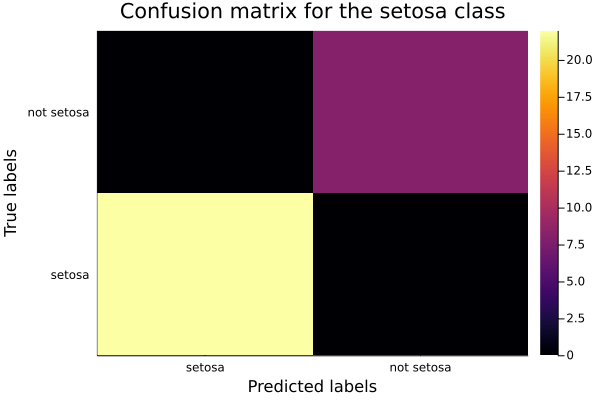
\includegraphics[scale=0.35]{../trab1 (simple perceptron)/figs/setosa-confusion-matrix.png}
    \caption{confusion matrix for setosa class.}
    \label{fig:confusion-matrix-setosa}
\end{figure}

The Figure \ref{fig:setosa-training-evolution} shows the evolution of the training dataset accuracy throughout the epochs. One can notice the fast convergence to the accuracy of 100\%.

\begin{figure}[H]
    \centering
    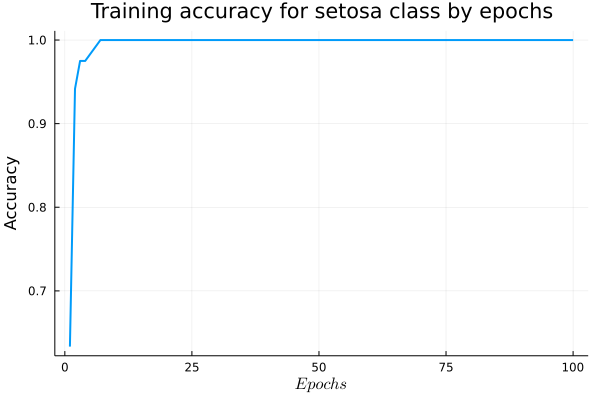
\includegraphics[scale=0.35]{../trab1 (simple perceptron)/figs/accuracy-by-epochs-for-setosa.png}
    \caption{Training dataset evolution for the setosa classification.}
    \label{fig:setosa-training-evolution}
\end{figure}

For a dummy dataset with \(K=4\) classes, the Rosenblatt's perceptron achieved a mean accuracy of 97.5\% and a standard deviation of 0.05. The Figure \ref{fig:decision-surface-dummy-data} shows the decision surface of the desired class for the realization whose accuracy is the closest to the mean accuracy. All instances of all classes are samples drawn from a Gaussian distribution with a given mean and variance.

\begin{figure}[H]
    \centering
    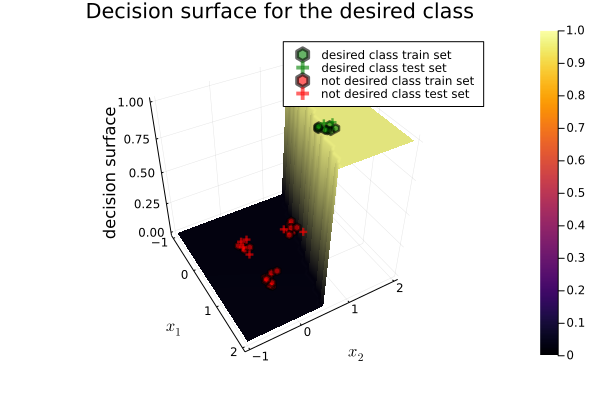
\includegraphics[scale=0.35]{../trab1 (simple perceptron)/figs/decision-surface-for-dummy-data.png}
    \caption{Decision surface for the desired class.}
    \label{fig:decision-surface-dummy-data}
\end{figure}

\section{ADALINE}

The Adaptive Linear Element (or ADALINE) is a variation of the Rosenblatt's perceptron, where the step function is replaced by a linear function, that is, \(y(n) = \varphi(u(n)) = u(n)\). One can combine a tapped delay line with an ADALINE, thus creating an adaptive filter, widely used in statistical signal processing.

Consider a regression problem where the desired signal comes from a function \(f(x)\) corrupted with Gaussian noise. The ADALINE model tries to retrieve the original data using the same process described in Algorithm \ref{alg:rosenblatt-perceptron}. However, the performance analysis is toward the MSE error instead the accuracy since it is now a regression problem.

The Table \ref{tab:adaline-results} shows the performance of the mean MSE and its standard deviation obtained over independent realizations, in addition to the root mean squared error (RMSE). We consider scenarios where \(f(\cdot)\) is a function of one or two variables. In other words, for the first scenario, the input is the vector
\begin{align}
    \begin{bmatrix}
        1 & x(n)
    \end{bmatrix} \in \Real^2
\end{align}
and \(f_1(x) = ax(n)+b\), while the input vector for the second scenario is given by
\begin{align}
    \begin{bmatrix}
        1 & x_1(n) & x_2(n)
    \end{bmatrix} \in \Real^3
\end{align}
and \(f_2(x_1, x_2) = ax_1(n)+bx_2(n)+c\).

\begin{table}[H]
	\centering
	\caption{ADALINE performance for regression problem}
	\footnotesize
	\setlength{\tabcolsep}{5pt}
	\begin{tabular}{ccccccccc}
		% \toprule [1.3pt]	
		% \multicolumn{4}{c}{ \textbf{Style} } \\
		\hline
		\(f(\cdot)\) & MSE mean & MSE standard deviation & RMSE mean & RMSE standard deviation \\
		\hline
		\(5x(n)+8\) & 9.69 & 2.84 & 3.07 & 0.47 \\
        \hline
		\(5x_1(n)+3x_2(n)+6\) & 9.93 & 4.27 & 3.08 & 0.66 \\
		\hline
	\end{tabular} \label{tab:adaline-results}
\end{table}

Naturally, both curves could be properly estimated since they are linear functions. The Figure \ref{fig:ADALINE-regression} shows the regression for the ADALINE model.

\begin{figure}[H]
    \centering

\subfloat[\centering ADALINE regression for \(5x+7\)]{%
  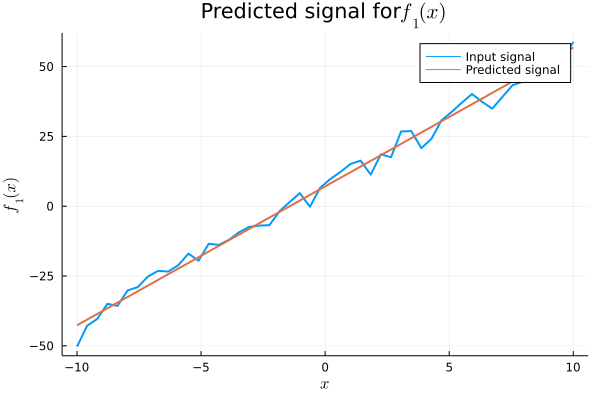
\includegraphics[clip,scale=0.4]{../trab2 (ADALINE)/figs/predict-f1.png}%
  \label{fig:itema}
}

\subfloat[\centering ADALINE regression for \(5x_1(n)+3x_2(n)+6\)]{%
  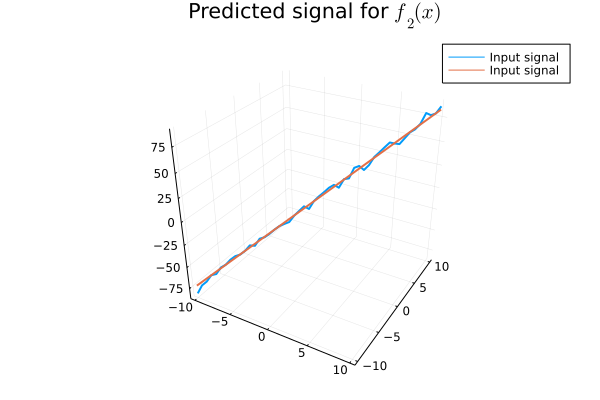
\includegraphics[clip,scale=0.5]{../trab2 (ADALINE)/figs/predict-f2.png}%
  \label{fig:itemb}
}

\caption{ADALINE regression}
\label{fig:ADALINE-regression}

\end{figure}

\section{Single Layer Perceptron}

Although Rosenblatt's perceptron can solve linear problems, it has only one output variable. A more reasonable model for a multivariate class problem is a single-layer perceptron (SLP) consisting of \(J\) neurons, where each neuron receives the same input signal, \(\mathbf{x}(n)\).

The matrix of all coefficients is given by
\begin{align}
    \mathbf{W}(n) = \begin{bmatrix}
        \mathbf{w}_1 (n)^\trans & \mathbf{w}_2 (n)^\trans & \cdots & \mathbf{w}_J (n)^\trans
    \end{bmatrix}^\trans \in \Real^{J \times \left(N_a+1\right)},
\end{align}
where \(J\) is the number of classes (one neuron for each class) and \(N_a\) is the number of attributes. The learning algorithm is given by
\begin{align}
    \mathbf{W}(n+1) = \mathbf{W}(n) + \eta \boldsymbol{\deltaup}(n) \mathbf{x}(n)^\trans,
\end{align}
where \(\boldsymbol{\deltaup}(n) = \begin{bmatrix}
    \delta_1(n) & \delta_2(n) & \delta_J(n)
\end{bmatrix}^\trans\) is the vector of the local gradients, being \(\delta_j(n)\) the local gradient of the \(j\)th perceptron. Let us define the vector of all induced local fields at the instant \(n\) as
\begin{align}
    \mathbf{v}(n) = \begin{bmatrix}
        v_1(n) & v_2(n) & v_J(n)
    \end{bmatrix}^\trans = \mathbf{W}(n) \mathbf{x}(n).
\end{align}

Notice that
\begin{align}
    \frac{\partial \mathscr{E}(n)}{\partial w_{ji}(n)} & = \frac{\partial \mathscr{E}(n)}{\partial v_{j}(n)} \frac{\partial v_j(n)}{\partial w_{ji}(n)} \nonumber \\
    & = - \delta_j (n) x_i(n),
    \label{eq:cost-function}
\end{align}
where
\begin{align}
    \frac{\partial v_j(n)}{\partial w_{ji}(n)} = x_i(n)
    \label{eq:chain4}
\end{align}
is the \(i\)th input at the instant \(n\), and
\begin{align}
    \delta_j (n) = - \frac{\partial \mathscr{E}(n)}{\partial v_{j}(n)} = - \frac{\partial \mathscr{E}(n)}{\partial e_{j}(n)} \frac{\partial e_j(n)}{\partial x_i(n)} \frac{\partial x_i(n)}{\partial v_{j}(n)}
    \label{eq:local-gradient}
\end{align}
is the local gradient of the \(j\)th neuron. In this equation, \(e_{j}(n)\) and \(v_{j}(n)\) are the error and the induced local field of the neuron \(j\), respectively, and \(w_{ji}(n)\) is the \(i\)th synaptic weight for the \(j\)th neuron at the instant \(n\).

Note also that
\begin{align}
    \frac{\partial \mathscr{E}(n)}{\partial e_{j}(n)} = e_{j}(n),
    \label{eq:chain1}
\end{align}

\begin{align}
    \frac{\partial e_j(n)}{\partial x_i(n)} = -1,
    \label{eq:chain2}
\end{align}
and
\begin{align}
    \frac{\partial x_i(n)}{\partial v_{j}(n)} \triangleq \varphi'(v_{j}(n)).
    \label{eq:chain3}
\end{align}
By substituting the equations \eqref{eq:chain1}, \eqref{eq:chain2}, and \eqref{eq:chain3} into \eqref{eq:local-gradient}, we get
\begin{align}
    \delta_j (n) = e_{j}(n) \varphi'(v_{j}(n)),
\end{align}
or in matricial notation,
\begin{align}
    \boldsymbol{\deltaup}(n) = \mathbf{e}(n) \odot \boldsymbol{\varphi}'(\mathbf{v}(n)),
\end{align}
where \(\odot\) is the Hadamard product and \(\boldsymbol{\varphi}'(\mathbf{v}(n)) = \begin{bmatrix}
    \varphi'(v_1(n)) & \varphi'(v_2(n)) & \cdots & \varphi'(v_K(n))
\end{bmatrix}^\trans\).

The synaptic weights update is given by
\begin{align}
    \Delta w_{ji}(n) = - \eta \frac{\partial \mathscr{E}(n)}{\partial w_{ji}(n)}.
    \label{eq:Delta_w_ji}
\end{align}
Substituting the Equation \eqref{eq:cost-function} into \eqref{eq:Delta_w_ji}, we have that
\begin{align}
    \Delta w_{ji}(n) = \eta \delta_j (n) x_i(n),
\end{align}
or in matricial notation
\begin{align}
    \Delta \mathbf{W}(n) = \eta\boldsymbol{\deltaup}(n) \mathbf{x}(n)^\trans.
\end{align}
Finally, the update function is given by
\begin{align}
    \mathbf{W}(n+1) & = \mathbf{W}(n) + \Delta \mathbf{W}(n) \nonumber \\
    & = \mathbf{W}(n) + \eta\boldsymbol{\deltaup}(n) \mathbf{x}(n)^\trans.
\end{align}

The Algorithm \ref{alg:single-layer-perceptron} summarizes the procedure of the SLP algorithm.

\begin{algorithm}[!ht]
    \DontPrintSemicolon
      
      \KwInput{\(\mathbf{X}, \mathbf{D}\) \tcc*{attributes and labels dataset}}
      
    %   \KwData{Testing set $x$}
      \ForAll{\(\left\{ 1, 2, \cdots, N_r \right\}\)}{
        \(\mathbf{W}(n) \leftarrow \text{initialize}\)

        \(\mathbf{X}, \mathbf{D} \leftarrow \text{shuffle}\)

        \( \left( \mathbf{X}_{trn}, \mathbf{D}_{trn} \right), \left( \mathbf{X}_{tst}, \mathbf{D}_{tst} \right)  \leftarrow \text{hold-out}\) \tcc{training and testing dataset}

        \ForAll{\(\left\{ 1, 2, \cdots, N_e \right\}\)}{
            \ForAll{Instancies in the training dataset}{
                \(\mathbf{v}(n) \leftarrow \mathbf{W}(n) \mathbf{x}(n)\)

                \(\mathbf{y}(n) \leftarrow \boldsymbol{\varphi}(\mathbf{v}(n))\)

                \(\mathbf{e}(n) \leftarrow \mathbf{d}(n) - \mathbf{y}(n)\)
            
                \(\boldsymbol{\deltaup}(n) \leftarrow \mathbf{e}(n) \odot \boldsymbol{\varphi}'(\mathbf{v}(n))\)

                \(\mathbf{W}(n+1) \leftarrow \mathbf{W}(n) + \eta\boldsymbol{\deltaup}(n) \mathbf{x}(n)^\trans\)
            }
            \(\mathbf{X}_{trn}, \mathbf{d}_{trn} \leftarrow \text{shuffle}\)
        }
        
        \(accuracy \leftarrow \text{test}(\mathbf{X}_{tst}, \mathbf{d}_{tst})\)
      }
    
    \caption{Single-layer perceptron}
    \label{alg:single-layer-perceptron}
\end{algorithm}

For the step function (MacCulloch and Pitts' activation function), its derivative does not exist, and the local gradient of the \(j\)th neuron is simply \(\delta_j(n) = e_j (n)\). For this classification problem, the labels were encoded using the one-hot method.

The Figure \ref{fig:heatmap-dummy-dataset} shows the heatmap for a dummy dataset consisting of \(K=3\) classes, \(N_a=2\) attributes, and \(N=150\) instances. The classifier used the MacCulloch and Pitts' activation function and achieved a mean accuracy of 99.49\% and a standard deviation of 0.0218. The same classifier was used for the iris dataset (\(K=3\) classe, \(N_a=4\) attributes, and \(N=150\) attributes) and the column dataset (\(K=3\) classes, \(N_a=6\) attributes, and \(N=310\) instances). For the iris dataset, the classifier achieved a mean accuracy of 88\% with a standard deviation of \(0.14\), while for the column dataset the model achieved a mean accuracy of 77.66\% with a standard deviation of \(0.06\).

\begin{figure}[H]
    \centering
    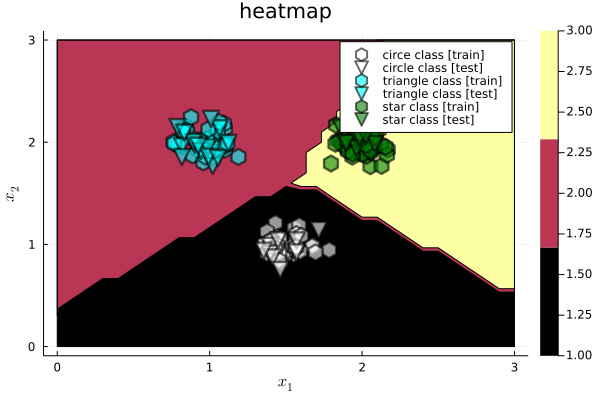
\includegraphics[scale=0.5]{../trab3 (single layer perceptron)/figs/dummy data - heatmap.png}
    \caption{Heatmap of the dummy dataset.}
    \label{fig:heatmap-dummy-dataset}
\end{figure}

Using the logistic function, the model achieved a mean accuracy of 100\% for the dummy data. The heatmap for this dataset is shown in Figure \ref{fig:dummy-data-heatmap}.


\begin{figure}[H]
    \centering
    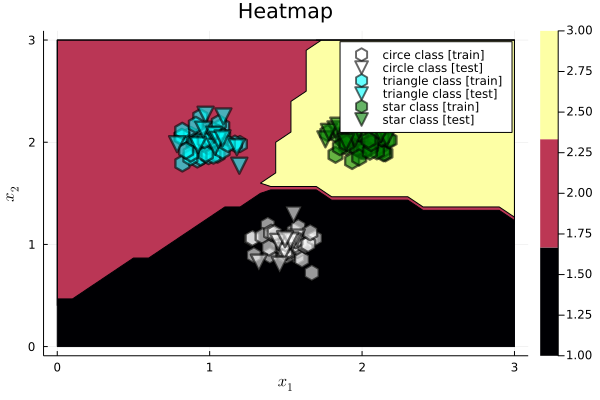
\includegraphics[scale=0.4]{../trab4 (single layer perceptron with sigmoidal functions)/figs/dummy data - heatmap.png}%
    
    \caption{The dummy dataset for the SLP with logistic activation function.}
    \label{fig:dummy-data-heatmap}
\end{figure}

For the iris dataset, SLP with logistic function reached a mean and a standard deviation of 87\% and 0.16, respectively.  The surface of decision for each class of iris data is shown in Figure \ref{fig:iris-decision-surface}. It is possible to notice that the classifier can solve the problem for the setosa class as it is linearly separable from the other classes for the attributes considered (petal length and petal width).

\begin{figure}[H]
    \centering
    \subfloat[\centering Setosa class]{%
      \includegraphics[scale=0.4]{../trab4 (single layer perceptron with sigmoidal functions)/figs/decision-surface-for-setosa.png}%
    }
    
    \subfloat[\centering Verginica class]{%
      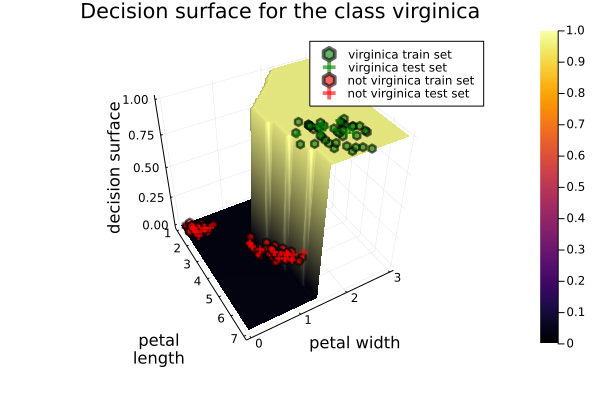
\includegraphics[scale=0.4]{../trab4 (single layer perceptron with sigmoidal functions)/figs/decision-surface-for-virginica.png}%
    }

    \subfloat[\centering Versicolor class]{%
      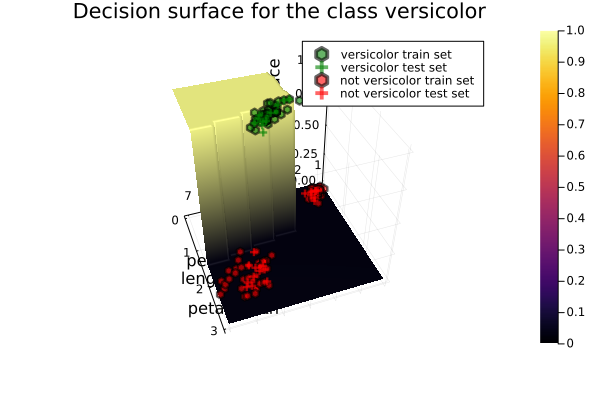
\includegraphics[scale=0.4]{../trab4 (single layer perceptron with sigmoidal functions)/figs/decision-surface-for-versicolor.png}%
    }
    
    \caption{The iris dataset for the SLP with logistic activation function.}
    \label{fig:iris-decision-surface}
    
\end{figure}

\section{Multilayer Perceptron}

Rosenblatt's perceptron and the single-layer perceptron use the LMS algorithm in the learning phase and are capable of estimating the gradient vector, which yields reasonable results for many problems. However, both architectures are restricted to the classification of linearly separable patterns.

To overcome the limitations of the aforementioned solutions, we introduce a new neural network structure, which employs \(L\) layers. This model is usually called Multilayer Perceptron (MLP). Each neuron uses a nonlinear activation function that is differentiable, and the final output can successfully solve nonlinear problems.

The presence of hidden layers makes the learning phase more complicated to devise since one must decide how the signal error should propagate toward the first layer. A popular learning algorithm used for MLP is the backpropagation algorithm, which in turn is rooted in the LMS algorithm.

The backpropagation algorithm entails two phases:
\begin{itemize}
    \item The \emph{forward phase}: at the instant \(n\), the synaptic weights of the network are fixed and the input signal, \(\mathbf{x}(n)\), is propagated from the input to the output layer. At each neuron, the induced local field is computed and the output of the activation function is delivered to each neuron located on the layer at its right.
    \item the \emph{backward phase}: signal error is produced at the output layer, where their weights are readily updated with the same procedure used in the SLP. Then, the synaptic weights of the hidden layers are updated, from the outmost hidden layer to the input layer, using the local gradients and the synaptic weights of the neurons on the layer at its right, in addition to the derivative of the activation function of the own neuron.
\end{itemize}

Since the update equation for the output layer was already derived in the SLP algorithm\footnote{The unique difference is that the input signal is \(\mathbf{y}^{(L-1)}(n)\) instead of \(\mathbf{x}(n)\)}, we will focus on finding the update equation of the \(l\)th hidden layer. Beginning with the outmost hidden layer and recalling that the local gradient of the \(j\)th neuron on this layer is given by
\begin{align}
    \delta_j^{(L-1)} (n) & = - \frac{\partial \mathscr{E}(n)}{\partial v_{j}^{(L-1)}(n)} \nonumber \\
    & = - \frac{\partial \mathscr{E}(n)}{\partial y_{j}^{(L-1)}(n)} \frac{\partial y_{j}^{(L-1)}(n)}{\partial v_{j}^{(L-1)}(n)} \nonumber \nonumber \\
    & = - \frac{\partial \mathscr{E}(n)}{\partial y_{j}^{(L-1)}(n)} \varphi'(v_j^{(L-1)}(n)),
    \label{eq:local-gradient}
\end{align}
where the third equation follows that
\begin{align}
    \varphi'(v_j^{(L-1)}(n)) = \frac{\partial y_{j}^{(L-1)}(n)}{\partial v_{j}^{(L-1)}(n)}.
\end{align}

We can derive the learning equation for this layer and generalize it to all hidden layers. In this section, a superscript was added to indicate which layer the signals refer to.

Remember that \(y_{j}^{(L-1)}(n)\) is the \(j\)th input signal on the output layer (\(L\)th layer), and that
\begin{align}
    \frac{\partial \mathscr{E}(n)}{\partial y_{j}^{(L-1)}(n)} = \sum_{k=1}^{m_L} e_k^{(L)}(n) \frac{\partial e_k^{(L)}(n)}{\partial y_{j}^{(L-1)}(n)},
\end{align}
where \(m_L\) is the number of neurons on the \(L\)th layer. By using the chain rule, we have that
\begin{align}
    \frac{\partial \mathscr{E}(n)}{\partial y_{j}^{(L-1)}(n)} = \sum_{k=1}^{m_L} e_k^{(L)}(n) \frac{\partial e_k^{(L)}(n)}{\partial v_{k}^{(L)}(n)} \frac{\partial v_{k}^{(L)}(n)}{\partial y_{j}^{(L-1)}(n)},
    \label{eq:partial-mlp}
\end{align}
but since \(e_k^{(L)}(n) = d_k^{(L)}(n) - \varphi(v_k^{(L)}(n))\), it follows that
\begin{align}
    \frac{\partial e_k^{(L)}(n)}{\partial v_{k}^{(L)}(n)} = - \varphi(v_k^{(L)}(n)).
    \label{eq:chain12}
\end{align}
Note that
\begin{align}
    v_{k}^{(L)} = \sum_{j=0}^{m_L} w_{kj}^{(L)}(n) y_{j}^{(L-1)}(n).
\end{align}
Therefore,
\begin{align}
    \frac{\partial v_{k}^{(L)}(n)}{\partial y_{j}^{(L-1)}(n)} = w_{kj}^{(L)}(n)
    \label{eq:chain22}
\end{align}
Substituting the Equations \eqref{eq:chain12} and \eqref{eq:chain22} into \ref{eq:partial-mlp}, we get
\begin{align}
    \frac{\partial \mathscr{E}(n)}{\partial y_{j}^{(L-1)}(n)}  & = - \sum_{k=1}^{m_L} e_k^{(L)}(n) \varphi(v_k^{(L)}(n)) w_{kj}^{(L)}(n) \nonumber \\
    & = - \sum_{k=1}^{m_L} \delta_k^{(L)} (n) w_{kj}^{(L)}(n),
    \label{eq:mlp-partial-final}
\end{align}
where the second equation follows that \(\delta_k^{(L)} = e_k^{(L)}(n) \varphi(v_k^{(L)}(n))\). Finally, substituting Equation \eqref{eq:mlp-partial-final} into \eqref{eq:local-gradient}, the local gradient of the \(j\)th neuron on the \((L-1)\)th hidden layer is given by
\begin{align}
    \delta_j^{(L-1)} (n) = \varphi'(v_j^{(L-1)}(n)) \sum_{k=1}^{m_L} \delta_k^{(L)} (n) w_{kj}^{(L)}(n),
\end{align}
or in matricial notation
\begin{align}
    \boldsymbol{\deltaup}^{(L-1)} (n) = \boldsymbol{\varphi}'(\mathbf{v}^{(L-1)}(n)) \odot \mathbf{W}^{(L)}(n) \boldsymbol{\deltaup}^{(L)} (n),
    \label{eq:uptade-layer-L-1}
\end{align}
The Equation \eqref{eq:uptade-layer-L-1} can be generalized to the \(l\)th layer:
\begin{align}
    \boldsymbol{\deltaup}^{(l)} (n) = \boldsymbol{\varphi}'(\mathbf{v}^{(l)}(n)) \odot \mathbf{W}^{(l+1)}(n) \boldsymbol{\deltaup}^{(l+1)} (n),
    \label{eq:uptade-layer-l}
\end{align}
where \(1\leq l < L\). The synaptic weights update is given by
\begin{align}
    \Delta \mathbf{W}^{(l)}(n) = \eta\boldsymbol{\deltaup}^{(l)}(n) \mathbf{y}^{(l-1)}(n)^\trans,
\end{align}
where \(\mathbf{y}^{(0)}(n) \triangleq \mathbf{x}(n)\). Therefore, the learning equation of the hidden layer is given by
\begin{align}
    \mathbf{W}^{(l)}(n+1) & = \mathbf{W}^{(l)}(n) + \Delta \mathbf{W}^{(l)}(n) \nonumber \\
    & = \mathbf{W}^{(l)}(n) + \eta\boldsymbol{\deltaup}^{(l)}(n) \mathbf{y}^{(l-1)}(n)^\trans.
\end{align}


The Algorithm \ref{alg:multilayer-perceptron} shows how the MLP uses the backpropagation algorithm.

\begin{algorithm}[H]
    \DontPrintSemicolon
      
      \KwInput{\(\mathbf{X}, \mathbf{D}\) \tcc*{attributes and labels dataset}}
      
    %   \KwData{Testing set $x$}
      \ForAll{\(\left\{ 1, 2, \cdots, N_r \right\}\)}{
        \(\mathbf{W}(n) \leftarrow \text{initialize}\)

        \(\mathbf{X}, \mathbf{D} \leftarrow \text{shuffle}\)

        \( \left( \mathbf{X}_{trn}, \mathbf{D}_{trn} \right), \left( \mathbf{X}_{tst}, \mathbf{D}_{tst} \right)  \leftarrow \text{hold-out}\) \tcc{training and testing dataset}

        \ForAll{\(\left\{ 1, 2, \cdots, N_e \right\}\)}{
            \ForAll{Instancies in the training dataset}{
                \tcc{forward phase}
                \For{\(l \in \left\{ 1, 2, ..., L \right\}\)}{
                    \(\mathbf{v}^{(l)}(n) \leftarrow \mathbf{W}^{(l)}(n) \mathbf{y}^{(l-1)}(n)\)

                    \(\mathbf{y}^{(l)}(n) \leftarrow \boldsymbol{\varphi}(\mathbf{v}^{(l)}(n))\)
                }
                
                \tcc{backward phase}
                
                \(\mathbf{e}(n) \leftarrow \mathbf{d}(n) - \mathbf{y}^{(L)}(n)\) \tcc*{output layer}
            
                \(\boldsymbol{\deltaup}^{(L)}(n) \leftarrow \mathbf{e}(n) \boldsymbol{\varphi}'(\mathbf{v}^{(L)}(n))\)

                \(\mathbf{W}^{(L)}(n+1) \leftarrow \mathbf{W}^{(L)}(n) + \eta\boldsymbol{\deltaup}^{(L)}(n) \mathbf{y}^{(L-1)}(n)^\trans\)

                \For{\(l \in \left\{ L-1, L-2, ..., 1 \right\}\)}{
                    \(\boldsymbol{\deltaup}^{(l)} (n) = \boldsymbol{\varphi}'(\mathbf{v}^{(l)}(n)) \odot \mathbf{W}^{(l+1)}(n) \boldsymbol{\deltaup}^{(l+1)} (n)\)
                }
            }
            \(\mathbf{X}_{trn}, \mathbf{d}_{trn} \leftarrow \text{shuffle}\)
        }
        
        \(accuracy \leftarrow \text{test}(\mathbf{X}_{tst}, \mathbf{d}_{tst})\)
      }
    
    \caption{Multilayer perceptron}
    \label{alg:multilayer-perceptron}
\end{algorithm}

\end{document}